\section{\cite{dornbusch1977comparative}: Continuum of Goods}

Consider a world economy with only two countries: Home and Foreign.
Use asterisks to denote foreign variables. 
\begin{note}
    \

    Ricardian models differ from other neoclassical trade models in that
    there is only \textbf{one factor of production} in the model.
\end{note}

We denote by:
\begin{itemize}
    \item $L$ and $L^*$ as the labor endowments in Home and Foreign respectively.
    \item $w$ and $w^*$ as the wages(in efficiency units) in Home and Foreign respectively.
\end{itemize}

There's a continuum of goods indexed by $z \in [0,1]$.
Since there are CRS, we can define the constant unit labot requirements in both countries: $a(z)$ and $a^*(z)$.

Without loss of generaliry, we order goods such that $A(z) \equiv \frac{a^*(z)}{a(z)}$ is decreasing.
\begin{itemize}
    \item Hence Home has a comparative advantage in goods with low-z goods.
    \item For simplicity, we'll assume strict monotonicity.
\end{itemize}

Previous supply-side assumptions are all we need to make qualitative
predictions about pattern of trade.

Let $p(z)$ denote the price of good $z$ in Home under free trade.

The profit-maximization condition for a firm producing good $z$ is:
\begin{align*}
    p(z) - w\,a(z) &\leq 0, \text{with equality if z produced at home.} \\
    p(z) - w^*\,a^*(z) &\leq 0, \text{with equality if z produced abroad.}  
\end{align*}
\begin{proposition}\label{prop:CA}
    \

    There exists $\tilde{z} \in [0,1]$, s.t. Home produces all goods with $z < \tilde{z}$ 
    and Foreign produces all goods with $z > \tilde{z}$.
\end{proposition}
\begin{proof}
    \

    By contradiction. Suppose that there exists $z^{\prime} < z$, s.t. $z$ produced at Home
    and $z^{\prime} $ is produced abroad. Then:
    \begin{align*}
        p(z) - w\,a(z) &= 0, \\
        p(z^{\prime}) - w\,a(z^{\prime}) &\leq 0, \\
        p(z^{\prime}) - w^*\,a^*(z^{\prime}) &= 0, \\
        p(z) - w^*\,a^*(z) &\leq 0.
    \end{align*}
    This implies that:
    \[w\,a(z)w^*\,a^*(z) = p(z)\,p(z^{\prime}) \leq w\,a(z^{\prime})\,w^*\,a^*(z),\]
    which can be rearranged as:
    \[\frac{a^*(z^{\prime})}{a(z^{\prime})} \leq \frac{a^*(z)}{a(z)}\]
    which contradicts that $A(z)$ is strictly decreasing.
\end{proof}

This proposition(\ref{prop:CA}) simply shows tha tHome should produce and specialize in
the goods in which it has a CA.

\begin{note}
    \

    \begin{itemize}
        \item Proposition(\ref{prop:CA}) doesn't rely on continuum of goods.
        \item Continuum of goods + continuity of $A(z)$ is important to derive the relative wage:
        \begin{equation}\label{eq:CA}
            A(\tilde{z}) = \frac{w}{w^*} \equiv \omega.
        \end{equation}
    \end{itemize}
    Equation(\ref{eq:CA}) is the key result of the Dornbusch, Fischer and Samuelson(1997) model.
    It gives us that: conditional on wages, goods should be produced in the country where it's cheaper to do so.
\end{note}

Then, we take a look at the demand side to pin down the relative wage $\omega$.
\subsection{Demand side}

Assume that consumers have identical Cobb-Douglas preferences around the world.

We denote by $b(z) \in (0,1)$ the share of expenditure spent on good $z$:
\[b(z) = \frac{p(z) c(z)}{wL} = \frac{p(z)c^*(z)}{w^* L^*}\]
where $c(z)$ and $c^*(z)$ are the consumption of good $z$ in Home and Foreign respectively.

By definition, share of expenditure satisfies: $\int_{0}^{1} b(z) dz = 1$.

Then, we denote by $\theta(\tilde{z}) = \int_0^{\tilde{z}} b(z) dz$ the fraction of income spent
on goods produced at Home(spent in both countries).

The trade balance requires: 
\[\theta(\tilde{z}) w^* L^* = [1-\theta (\tilde{z})]wL\]
where LHS od the Home exports an d RHE is the Home imports.

WE can then rearrange the equation(\ref{eq:CA}) to get:
\begin{equation}
    \omega  = \frac{\theta(\tilde{z})}{1 - \theta(\tilde{z})}\Bigl(\frac{L^*}{L}\Bigr) \equiv B(\tilde{z}).
\end{equation}

Note that $B^{\prime} > 0$ and: an increase in $\tilde{z}$ leads to a trade surplus at Home,
which must be compensated by an increase in Home's relative wage $\omega$.

\tikzset{every picture/.style={line width=0.75pt}} %set default line width to 0.75pt        

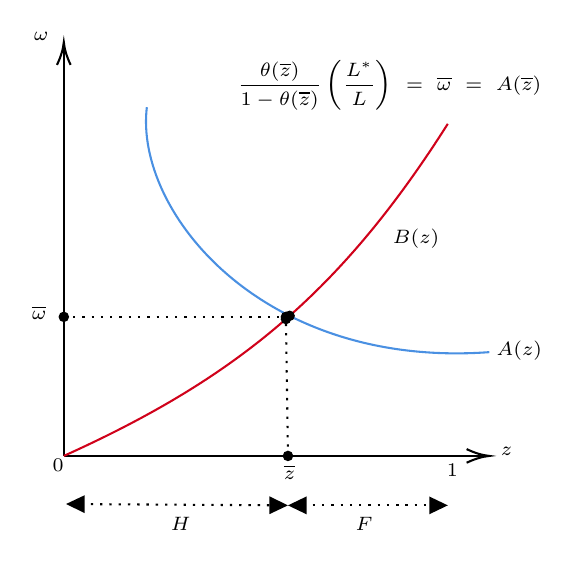
\begin{tikzpicture}[x=0.75pt,y=0.75pt,yscale=-1,xscale=1]
%uncomment if require: \path (0,300); %set diagram left start at 0, and has height of 300

%Straight Lines [id:da6380191506568016] 
\draw    (78.91,229.83) -- (78.91,32.5) ;
\draw [shift={(78.91,30.5)}, rotate = 90] [color={rgb, 255:red, 0; green, 0; blue, 0 }  ][line width=0.75]    (10.93,-3.29) .. controls (6.95,-1.4) and (3.31,-0.3) .. (0,0) .. controls (3.31,0.3) and (6.95,1.4) .. (10.93,3.29)   ;
%Straight Lines [id:da38275432146335675] 
\draw    (78.91,229.83) -- (281.91,229.83) ;
\draw [shift={(283.91,229.83)}, rotate = 180] [color={rgb, 255:red, 0; green, 0; blue, 0 }  ][line width=0.75]    (10.93,-3.29) .. controls (6.95,-1.4) and (3.31,-0.3) .. (0,0) .. controls (3.31,0.3) and (6.95,1.4) .. (10.93,3.29)   ;
%Curve Lines [id:da9974954988232241] 
\draw [color={rgb, 255:red, 208; green, 2; blue, 27 }  ,draw opacity=1 ]   (78.91,229.83) .. controls (160.91,192.83) and (211.91,151.83) .. (263.91,69.83) ;
%Curve Lines [id:da921906449816945] 
\draw [color={rgb, 255:red, 74; green, 144; blue, 226 }  ,draw opacity=1 ]   (118.91,61.83) .. controls (112.91,111.83) and (173.91,187.83) .. (283.91,179.83) ;
%Straight Lines [id:da49907072844197875] 
\draw  [dash pattern={on 0.84pt off 2.51pt}]  (78.91,162.83) -- (185.91,162.83) ;
%Straight Lines [id:da04673978660389] 
\draw  [dash pattern={on 0.84pt off 2.51pt}]  (186.91,229.83) -- (185.91,162.83) ;
%Straight Lines [id:da23882778580283293] 
\draw  [dash pattern={on 0.84pt off 2.51pt}]  (83,253.02) -- (183.91,253.63) ;
\draw [shift={(186.91,253.65)}, rotate = 180.35] [fill={rgb, 255:red, 0; green, 0; blue, 0 }  ][line width=0.08]  [draw opacity=0] (8.93,-4.29) -- (0,0) -- (8.93,4.29) -- cycle    ;
\draw [shift={(80,253)}, rotate = 0.35] [fill={rgb, 255:red, 0; green, 0; blue, 0 }  ][line width=0.08]  [draw opacity=0] (8.93,-4.29) -- (0,0) -- (8.93,4.29) -- cycle    ;
%Straight Lines [id:da7231487759136938] 
\draw  [dash pattern={on 0.84pt off 2.51pt}]  (189.91,253.65) -- (260.91,253.65) ;
\draw [shift={(263.91,253.65)}, rotate = 180] [fill={rgb, 255:red, 0; green, 0; blue, 0 }  ][line width=0.08]  [draw opacity=0] (8.93,-4.29) -- (0,0) -- (8.93,4.29) -- cycle    ;
\draw [shift={(186.91,253.65)}, rotate = 0] [fill={rgb, 255:red, 0; green, 0; blue, 0 }  ][line width=0.08]  [draw opacity=0] (8.93,-4.29) -- (0,0) -- (8.93,4.29) -- cycle    ;

% Text Node
\draw (62,156) node [anchor=north west][inner sep=0.75pt]  [font=\scriptsize] [align=left] {$\displaystyle \overline{\omega }$};
% Text Node
\draw (183.41,232.83) node [anchor=north west][inner sep=0.75pt]  [font=\scriptsize] [align=left] {$\displaystyle \overline{z}$};
% Text Node
\draw (286,173) node [anchor=north west][inner sep=0.75pt]  [font=\scriptsize] [align=left] {$\displaystyle A( z)$};
% Text Node
\draw (236,119) node [anchor=north west][inner sep=0.75pt]  [font=\scriptsize] [align=left] {$\displaystyle B( z)$};
% Text Node
\draw (63,24) node [anchor=north west][inner sep=0.75pt]  [font=\scriptsize] [align=left] {$\displaystyle \omega $};
% Text Node
\draw (288,224) node [anchor=north west][inner sep=0.75pt]  [font=\scriptsize] [align=left] {$\displaystyle z$};
% Text Node
\draw (72,230) node [anchor=north west][inner sep=0.75pt]  [font=\scriptsize] [align=left] {$\displaystyle 0$};
% Text Node
\draw (129,258) node [anchor=north west][inner sep=0.75pt]  [font=\scriptsize] [align=left] {$\displaystyle H$};
% Text Node
\draw (218,258) node [anchor=north west][inner sep=0.75pt]  [font=\scriptsize] [align=left] {$\displaystyle F$};
% Text Node
\draw (262,232) node [anchor=north west][inner sep=0.75pt]  [font=\scriptsize] [align=left] {$\displaystyle 1$};
% Text Node
\draw (161,38) node [anchor=north west][inner sep=0.75pt]  [font=\scriptsize] [align=left] {$\displaystyle \frac{\theta (\overline{z})}{1-\theta (\overline{z})}\left(\frac{L^{*}}{L}\right) \ =\ \overline{\omega } \ =\ A(\overline{z})$};

\draw [fill={rgb, 255:red, 0; green, 0; blue, 0 }  ,fill opacity=1 ]  (187.7, 162.33) circle [x radius= 2, y radius= 2]   ;
\draw [fill={rgb, 255:red, 0; green, 0; blue, 0 }  ,fill opacity=1 ]  (78.91, 162.83) circle [x radius= 2, y radius= 2]   ;
\draw [fill={rgb, 255:red, 0; green, 0; blue, 0 }  ,fill opacity=1 ]  (185.91, 162.83) circle [x radius= 2, y radius= 2]   ;
\draw [fill={rgb, 255:red, 0; green, 0; blue, 0 }  ,fill opacity=1 ]  (186.91, 229.83) circle [x radius= 2, y radius= 2]   ;
\draw [fill={rgb, 255:red, 0; green, 0; blue, 0 }  ,fill opacity=1 ]  (185.93, 163.89) circle [x radius= 2, y radius= 2]   ;
\end{tikzpicture}


\begin{itemize}
    \item Efficient international specialization, Equation (3), and trade balance, (4), jointly determine $(\bar{z}, \bar{\omega})$
\end{itemize}

Since Ricardian model is a neoclassical model, general results derived
in previous lecture hold. However, we can directly show the existence of gains from trade in this environment.

\begin{itemize}
    \item Set $w=1$ under autarky and free trade.
    \item Indirect utility\footnote{The maximum utility under budget constraint.} of Home representative houssehold depends on $p(\cdot).$
    \item For goods $z$ produced at Home under free trade: no change sompared to autarky.
    \item For goods $z$ produced Foreign under free trade:
    \[p(z) = w^* a^*(z) < a(z)\]
    \item Since all prices go down, indirect utility must go up.
\end{itemize}

\subsection{Consequences of (Relative) Country Growth}

Suppose that $L^*/L$ increases, then the relative wage $\omega$ must increase and $\tilde{z}$ goes down.
At initial wages, an increase in $L^*/L$ leads to a trade deficit in Foreign, which must be compensated by an increase in $\omega$.

An increase in $L^*/L$ raises indirect utility, i.e. real wage, of representative household at Home and lowers it in Foreign.

\begin{itemize}
    \item We set $w=1$ before and after the change in $L^*/L.$
    \item For goods $z$ whose production remains at Home, there's no change in $p(z)$.
    \item For goods $z$ whose production remains in Foreign, we have: $w \uparrow \Rightarrow w^* \downarrow \Rightarrow p(z) = w^* a^*(z) \downarrow.$
    \item For goods $z$ whose production changes from Home to Foreign, we have: $p(z) = w^* a^*(z) \leq a(z) \Rightarrow p(z) \downarrow.$
    \item So Home gains. Similar logic implies Foreign welfare loss.
\end{itemize}

\begin{note}
    \
    
    In spite of CRS at the industry level, everything is as if we had DRS at the country-level.

    As foreing's size increases, it specialized in sectors in which it is relatively less productive(compared to home),
    which worsens it's terms of trade, so lowers real GDP per capita.

    The flatter the A schedule, the smaller this effect.
\end{note}

If there's an improvement in Home technology, then unit of labor requirement in Home $a(z)$ will be reducing, hence $A(z)$ is increasing - shifting upward. 
As we have shown in \ref{eq:CA}, this shows \textbf{an increase in home relative wage} i.e. higher income, 
and \textbf{an increase in home's share of world production and trade.}\footnote{As shown previously, $\omega = \frac{\theta(\tilde{z})}{1-\theta(\tilde{z})} \Bigl(\frac{L^*}{L}\Bigr)$, 
if $\omega$ increases, and we fix $\frac{L^*}{L}$, then $\theta(\tilde{z})$ increases.} 

\section{\cite{eaton2002technology}: Many Countries}
The model of \cite{dornbusch1977comparative} is based on the Ricardian model
where trade and specialization patterns are determined by different productivities.

In the Dornbusch-Fischer-Samuelson model, there were no restrictions on the productivity distributions,
Eaton and Kortum were able to extent the model to a case with many countries by sacrificing this generality.

The Eaton-Kortum model is based on the following assumptions:
\begin{itemize}
    \item Perfect Competition
    \item $N$ countries, insteat of 2 in DFS
    \item Continuum of goods $(u \in [0,1])$
    \item CRS technology: labor only
    \item CES preferences with elasticity of substitution $\sigma > 0$
\end{itemize}

\subsection{Model Setup}

\subsubsection{The world}

In this model, there a finite number of countries $i \in S \equiv \{1, \cdots, N\}$; 
(unlike previous models, there are technical difficulties in extending the model to a continuum of countries).
There are a continuum of goods $\Omega$.

However, unlike \cite{krugman1980scale} and \cite{melitz2003impact}, models which follow(in Lecture 4 and 5),
\textit{every country is able to produce every good.}
Countries, however, varies(exogeneously) in their productivity of each good $z_i(\omega)$ - varying by country $i$ and good $\omega \in \Omega$.

The \cite{eaton2002technology} has no concept of a firm. Instead, it is assumed that all
goods $\omega$ are are produced using the same bundle of inputs with a constant returns to
scale technology. Let the cost of a bundle of inputs in country $i$ be $c_i$,
so that the cost of producing one unit of $\omega \in \Omega$ in country $i$ is $\frac{c_i}{z_i(\omega)}$.

Firstly, we introduce the \textbf{trade costs}: transport costs and tariffs. This is not an innovation of Eaton
and Kortum, the original Dornbush-Fischer-Samuelson model also had trade costs, but for simplification, we left them out.
    
Trade costs are modelled as iceberg costs, a popular device invented by Samuelson\cite{samuelson1954transfer}.
That is, we assume that for delivering one unit of a good from country $i$ to country $j$, 
it's necessary to ship $d_{ij} \geq 1$ units of good: the rest “melts away” during transit. 

\subsubsection{Supply}

Each good is assumed to be sold in perfectly competitive markets, so that the price a
consumer in country $j$ would pay for good $\omega$ produced in country $i$ is given by:
\begin{gather*}
    p_{ij}(\omega) = \frac{c_i}{z_i(\omega)} d_{ij}. \label{eq:EKprice}
\end{gather*}

However, consumers in country $j \in S$ are assumed to only purchase good $\omega \in \Omega$
from the country who can provide it at the lowest price, so the price a consumer in
$j \in N$ actually pays for good $\omega$ is:
\begin{gather*}
    p_j(\omega) = \min_{i \in S} p_{ij}(\omega) = \min _{i \in S} \Bigl\{ \frac{c_i}{z_i(\omega)} d_{ij} \Bigr\} \label{eq:EKprice2}
\end{gather*}

Here, the basic idea of Eaton and Kortum is already present in equation above:
a country $j \in S$ is more likely to purchase a good $\omega \in \Omega$ from country $i \in S$ if
\begin{enumerate}
    \item[(1)] it has a lower cost $c_i$;
    \item[(2)] it has a higher good productivity $z_i(\omega)$;
    \item[(3)] it has a lower trade cost $d_{ij}$. 
\end{enumerate}

\textbf{The main innovation of Eaton and Kortum}, however, is to assume that the productivities $z_i(\omega)$ are drawn from a Fréchet distribution\footnote{To find more properties of the Fréchet distribution, see the appendix \ref{sec:frechet}.}.
This means that for each $i \in S$ and $\forall \omega \in \Omega$, the cumulative distribution function $F_i$ is:
\[
F_i(z) = \operatorname{Pr}\Bigl\{z_i(\omega) \leq z \Bigr\} = \exp \Bigl\{-T_i z^{-\theta} \Bigr\}
\]
where $T_i > 0$ is a measure of the aggregate productivity of country $i$(country $i$'s state of technology), and $\theta>1$, 
which measures teh intra-industry heterogrneity, idiosyncratic variation in know-how across goods $\rightarrow$ drive intra-industry trade(comparative advantage).\footnote{A larger value of $T_i$ decreases $F_i$ fro any $z\geq 0$. It increases the probability of larger values
of $z$ and $\theta>1$, which is assumed to be constant across countries, governs the distribution of productivities across goods within countries. As $\theta$ increases, the heterogeneity of productivity across goods declines.}.
\begin{itemize}
    \item High $\theta$ means less variability and less intra-industry trade;
    \item It's important to assume that $\theta$ is common across industries;
    \item $\theta$ guides the impact of changes in fundamental productivity on aggregate trade flows.
\end{itemize}


\begin{note}[Why Fréchet?]
    \

    Why make this particular distributional assumption for productivities?

    \cite{kortum1997research} showed that if the technology of producing goods is determined by
    the best ``idea'' of how to produce, then the limiting distribution is indeed Fréchet, where
    $T_i$ reflects the country`s stock of ideas. More generally, consider the random variable:
    \[
    M_n = \max \{X_1, \cdots, X_n \}
    \]
    where $X_n$ are i.i.d.

    The Fisher-Tippett-Gnedenko theorem states that the only (normalized) distribution of
    $M_n$ as $n \to \infty $ is an extreme value distribution, of which Fréchet is one of three types (Type II).
    Note that a conditional logit model assumes that the error term is Gumbel (Type I) extreme value distributed.

    If random variable $x$ is Gumbel distributed, then $\ln{x}$ is Fréchet distributed. Hence, loosely speaking,
    the Fréchet distribution works better for models that are log linear (like the gravity equation), whereas the Gumbel
    distribution works better for models that are linear.
\end{note}

\subsubsection{Demand}

As in previous models, consumers have CES preferences so that the representative agent
in country $j$ has utility:
\[
U_j = \Bigl( \int_{\Omega} q_j(\omega)^{\frac{\sigma -1}{\sigma}} d \omega \Bigr)^{\frac{\sigma}{\sigma-1}},
\]
where $q_j(\omega)$ is the quantity that country $j$ consumes of good $\omega$.

Note that unlike the Krugman (1980)\cite{krugman1980scale} model, not every good produced in every country will be sold to country $j$.

Indeed, good $\omega \in \Omega$ will be produced by all countries but country $j$ will only purchase
it from one country. The CES preferences will yield a Dixit-Stiglitz price index:
\[
P_j \equiv \Bigl( \int_{\Omega} p_j(\omega)^{1-\sigma} \Bigr)^{\frac{1}{1-\sigma}}.
\]

\subsection{Equilibrium}

We now consider the equilibrium of the model. Instead of relying on the CES demand
equation as in the previous models, we use a probabilistic formulation in order to solve
the model.

\subsubsection{Prices}

In perfect competition only the lowest cost producer of a good will supply that particular
good. Thus, we want to derive the distribution of the minimum price over a set of prices
offered by producers in different countries:
\[
p_j = \min \{p_{ij}, \cdots, p_{Nj} \}.
\]
In order to solve the model, we take advantage of the properties of the Fréchet distribution.

First, we consider the probability that country $i \in S$ is able to offer country $j$ good $\omega$
for a price less than $p$. Because the technology is i.i.d. across goods, we can define:
\begin{gather*}
    G_{ij}(p) \equiv \operatorname{Pr} \Bigl\{ p_{ij}(\omega) \leq p \Bigr\}
\end{gather*}
Using the perfect competition price equation(\ref{eq:EKprice}), we can write:
\begin{align*}
    G_{ij}(p) &= \operatorname{Pr} \Bigl\{ \frac{c_i}{z_i(\omega)} d_{ij} \leq p \Bigr\} \\
    &= 1 - \operatorname{Pr} \Bigl\{ z_i(\omega) \geq \frac{c_i d_{ij}}{p} \Bigr\} \\
    &= 1 - F_i \Bigl( \frac{c_i d_{ij}}{p} \Bigr) \\
    &= 1 - \exp \Bigl\{ -T_i \Bigl( \frac{c_i d_{ij}}{p} \Bigr)^{-\theta} \Bigr\}
\end{align*}
Consider now the probability that country $j$ pays a price less than $p$ for good $\omega $.

Again, because the technology is i.i.d. across goods, the probability will be tha same fo all goods $\omega \in \Omega$.
Define:
\begin{gather}
    G_j(p) \equiv \operatorname{Pr} \Bigl\{ p_j(\omega) \leq p \Bigr\}
\end{gather}
Because country $j$ buys from the least cost provider, using equation \ref{eq:EKprice2}, we can write:
\begin{align*}
    G_j(p) &= \operatorname{Pr} \Bigl\{ \min_{i \in S} p_{ij}(\omega) \leq p \Bigr\} \\
    &= 1 - \operatorname{Pr} \Bigl\{ \min_{i \in S} p_{ij}(\omega) \geq p \Bigr\} \\
    &= 1 - \operatorname{Pr} \Bigl\{ \cap_{i \in S} \Bigl( p_{ij}(\omega) \geq p \Bigr) \Bigr\} \\
    &= 1 - \prod_{i \in S} \operatorname{Pr} \Bigl\{ p_{ij}(\omega) \geq p \Bigr\} \\
    &= 1 - \prod_{i \in S} \Bigl( 1 - G_{ij}(p) \Bigr)
\end{align*}
Substituting $G_{ij}$ into this equation, we have:
\begin{align*}
    G_j(p) &= 1 - \prod_{i \in S} \Bigl( 1 - \Bigl( 1 - \exp \Bigl\{ -T_i \Bigl( \frac{c_i d_{ij}}{p} \Bigr)^{-\theta} \Bigr\} \Bigr) \Bigr) \\
    &= 1 - \prod_{i \in S} \exp \Bigl\{ -T_i \Bigl( \frac{c_i d_{ij}}{p} \Bigr)^{-\theta} \Bigr\} \\
    &= 1 - \exp \Bigl\{ -p^{\theta} \sum_{i \in S} T_i \Bigl( c_i d_{ij} \Bigr)^{-\theta} \Bigr\} \\
    &= 1 - \exp \Bigl\{-p^{\theta} \Phi_j \Bigr\}
\end{align*}
where $\Phi_j = \sum_{i \in S} T_i (c_i d_{ij})^{-\theta}$. 

This tells us the distribution of prices across goods in country $j$.
This will further allow us to calculate the price index $P_j$ for country $j$.
\begin{align*}
    P_j &= \Bigl( \int_{\Omega}p_j(\omega)^{1-\sigma} \Bigr)^{\frac{1}{1-\sigma}} \\
    \Leftrightarrow P_j^{1-\sigma} &= \int_0^{\infty} p^{1-\sigma} d G_j(p)\\
    &= \int_0^{\infty} p^{1-\sigma} \Phi_j \exp \Bigl\{-p^{\theta} \Phi_j \Bigr\} dp \\
    &= \theta \Phi_j \int_0^{\infty} p^{\theta - \sigma} \exp \Bigl\{-p^{\theta} \Phi_j \Bigr\} dp.
\end{align*}
Define $x = p^{\theta} \Phi_j$, so $dx = \theta \Phi_j p^{\theta-1} dp$,with a change of variable, we have:
\begin{align*}
    P_j^{1-\sigma} &= \int_0^{\infty} \Bigl( \frac{x}{\Phi_j} \Bigr)^{\frac{1-\sigma}{\theta}} \exp\{-x\} dx \\
    &= \Phi_j^{-\frac{1-\sigma}{\theta}} \int_0^{\infty} x^{\frac{1-\sigma}{\theta}} \exp\{-x\} dx \\
    &= \Phi_j^{-\frac{1-\sigma}{\theta}} \Gamma \Bigl( \frac{1-\sigma}{\theta} + 1 \Bigr) \\
    \Leftrightarrow P_j &= \Phi_j^{-\frac{1}{\theta}} \Gamma \Bigl( \frac{\theta + 1 - \sigma}{\theta} \Bigr)^{\frac{1}{1-\sigma}}
\end{align*}
where $\Gamma(x) = \int_0^{\infty} x^{t-1} e^{-x} dx$ is the gamma function.

Hence, the equilibrium price index for a CES utililty with elasticity of substitution $\sigma < 1+\theta$ in country $j \in N$ can be written as:
\[
P_j = \gamma \Bigl( \sum_{i \in S} T_i (c_i d_{ij})^{-\theta} \Bigr)^{-\frac{1}{\theta}} 
\]
where $\gamma \equiv \Gamma \Bigl( \frac{\theta + 1 - \sigma}{\theta} \Bigr)^{\frac{1}{1-\sigma}}$ is a constant.

\subsection{Gravity}

What is the probability that a country $i$ actually buys a good $\omega$ from another country $j$?

Because all goods receive i.i.d. draws and there are a continuum of varieties, 
by the law of large numbers, this probability will be equal to the fraction of goods $i$ sells to $j$.

\begin{align*}
    \pi_{ij} &= \operatorname{Pr} \Big\{ p_{ij}(\omega) \leq \min_{k \in S \setminus j} p_{kj}(\omega) \Bigr\} \\
    &= \int_0^{\infty} \operatorname{Pr} \Bigl\{ p \leq \min_{k \in S \setminus j} p_{kj}(\omega) \Bigr\} d G_{ij}(p) \\ 
    &= \int_0^{\infty} \operatorname{Pr} \Bigl\{\cap_{k \in S \setminus j} (p_{kj}(\omega) \geq p) \Bigr\} d G_{ij}(p) \\
    &= \int_0^{\infty} \prod_{k \in S \setminus j} \Bigl(1 - G_{kj}(p) \Bigr) d G_{ij}(p)
\end{align*}

Substituting the distribution of price yields:
\begin{align*}
    \pi_{ij} &= \int_0^{\infty} \prod_{k \in S \setminus j} (1 - G_{kj}(p)) \, d G_{ij}(p) \\
    &= \int_0^{\infty} \prod_{k \in S \setminus j} (1 - \exp\{-p^{\theta} \Phi_k\}) \, d G_{ij}(p) \\
    &= \int_0^{\infty} \prod_{k \in S \setminus j} \Bigl( \exp\Bigl\{-T_k \Bigl(\frac{c_k d_{kj}}{p}\Bigr)^{-\theta} \Bigr\} \Bigr) \Bigl( \pd{}{p} \Bigl( 1 - \exp \Bigl\{ -T_i \Bigl(\frac{c_i d_{ij}}{p}\Bigr)^{-\theta} \Bigr\} \Bigr) \Bigr) dp \\
    &= T_i (c_i d_{ij})^{-\theta} \int_0^{\infty} \theta p^{\theta-1} \exp \Bigl\{ \sum_k -T_k \Bigl( \frac{c_k d_{kj}}{p} \Bigr)^{-\theta} \Bigr\} dp \\
    &= T_i (c_i d_{ij})^{-\theta} \int_0^{\infty} \theta p^{\theta -1} \exp \Bigl\{-p^{\theta \Phi_j} \Bigr\} dp \\
    &= \frac{T_i (c_i d_{ij})^{-\theta} }{\Phi_j} \int_0^{\infty} \theta p^{\theta-1} \Phi_j \exp \Bigl\{-p^{\theta} \Phi_j \Bigr\} dp \\
    &= \frac{T_i (c_i d_{ij})^{-\theta} }{\Phi_j} \cdot -\exp \Bigl\{-p^{\theta} \Phi_j \Bigr\} \Bigg| _{p=0}^{\infty} \Bigg. \\
    &= \frac{T_i (c_i d_{ij})^{-\theta} }{\Phi_j}
\end{align*}
Hence, the fraction of goods exported form $i$ to $j$ just depends on $i$'s share on $j$'s $\Phi_j$.

\begin{intuition}
    \

    Intuitively, $\pi_{ij}$ is increasing in $T_j$: if country $j$ is on average more productive, then country $i$ will import a lot from $j$;
    but decreasing in $c_i$ and $d_{ij}$: if country $j$ is more expensive in wages or trade costs are higher, then it's a less attractive source of imprts to country $i$.
\end{intuition}

\begin{note}[More about the Fréchet Distribution]
    \

    $\pi_{ij}$ is the fraction of goods that $j$ purchases from $i$, it may not be the fraction of $j$'s income that is spent on goods from country $i$.
    However, it turns out that with Fréchet distribution, \textit{the distribution of prices of goods that country $j$ actually
    purchases from any country $i \in S$ will be the same.}
\end{note}

Intuitively, what is happening is that origins with better comparative advantage (lower
trade costs, better productivity, etc.) in selling to $j$ will exploit its advantage by 
selling a greater number of goods to $j$ exactly up to the point where the distribution
of prices it offers to $j$ is the same as $j$'s overall price distribution.

While the result depends heavily on the Fréchet distribution, the distribution of prices offered 
to an importing country $j$ is independent from the origin, country $j$'s average expenditure per good
doesn't depend on the source of the good.

As a result, the fraction of goods purchased from a particular origin $i$, denoted by $\pi_{ij}$, 
is equal to the fraction of $j$'s income spent on goods form $i$:
\begin{gather}
    \lambda_{ij} \equiv \frac{X_{ij}}{Y_j} = \frac{T_i (c_i d_{ij})^{-\theta}}{\Phi_j} \label{eq:EKfraction}
\end{gather}
This implies that the total expenditure of $j$ on goods from country $i$ is:
\[X_{ij} = \pi_{ij} E_j \Rightarrow X_{ij} = \frac{T_i (c_i d_{ij})^{-\theta}}{\Phi_j} E_j.\]
Suppose that $c_i = w_i$ and substitute into the price index, yields:
\[
X_{ij} = \gamma^{-\theta} d_{ij}^{-\theta} w_i^{-\theta} T_i E_j P_j^{\theta}.
\]
As in previous models, we can also push the gravity equation a little bit further. Note
that in general equilibrium, the total income of a country will equal the amount it sells to
all other countries:
\[
Y_i = \sum_{j \in S} X_{ij} 
\]
Substitute $X_{ij}$ into $Y_i$, yields:
\begin{align*}
    Y_i &= \sum_{j \in S} \gamma^{-\theta} d_{ij}^{-\theta} w_i^{-\theta} T_i E_j P_j^{\theta} \\
    &= \gamma^{-\theta} w_i^{-\theta} T_i \sum_{j \in S} d_{ij}^{-\theta} E_j P_j^{\theta} \\
    \Leftrightarrow \gamma^{-\theta} w_i^{-\theta} T_i &= \frac{Y_i}{\sum_{j \in S} d_{ij}^{-\theta} E_j P_j^{\theta}}
\end{align*}
Thus, we can write the gravity equation in a more general form:
\begin{align*}
    X_{ij} &= \gamma^{-\theta} d_{ij}^{-\theta} w_i^{-\theta} T_i E_j P_j^{\theta} \\
    &= d_{ij}^{-\theta} \times \frac{Y_i}{\Omega^{-\theta}} \times \frac{E_j}{P_j^{-\theta}}
\end{align*}
where $\Omega_i \equiv \Bigl( \sum_{k \in S} d_{ik}^{-\theta} \frac{E_k}{P_k^{-\theta}}\Bigr)^{-\frac{1}{\theta}}$.
We will see soon that if trade costs are symmetric, $\Omega_i = P_i$.

\begin{note}[Notation in Lecture slide]
    \

    Denote total spending in country $i$ on goods from country $j$ as $X_{ij}$;
    country $i$`s total spending on all goods as $X_i \equiv \sum_j X_{ij}$.

    We know that $\frac{X_{ij}}{X_i} = \pi_{ij}$, so
    \[
    X_{ij} = \frac{T_j (c_j d_{ij})^{-\theta}}{\Phi_i} X_i
    \]
    Let $Y_j = \sum_i X_{ij}$ be country $j$'s total sales, then we can write:
    \[
    Y_j = \sum_i \frac{T_j (c_j d_{ij})^{-\theta} X_i}{\Phi_i} = T_j c_j^{-\theta} \Omega_j^{-\theta}
    \]
    where $\Omega_j = \sum_i d_{ij}^{-\theta} \frac{X_i}{P_i^{-\theta}}$ is the average price index of country $i$.

    Solving $T_j c_j^{-\theta}$ from $Y_j = T_j c_j^{-\theta} \Omega_j^{-\theta}$ and plug into $X_{ij}$,
    \[
    X_{ij} = \frac{X_i Y_j d_{ij}^{-\theta} }\Omega_i^{\theta}{\Phi_i}.
    \]
    Ug $p_i = \gamma \Phi_i^{\frac{1}{\theta}}$, we get:
    \[
    X_{ij} = \gamma^{-\theta} X_i Y_j d_{ij}^{-\theta} (p_i \Omega_j)^{\theta}. \label{eq:EKgravity}
    \]
\end{note}

\begin{remark}
    \

    In this model, changes in trade costs affect the extensive margin, i.e. which goods an origin country trades with a destination country. 
    As the bilateral trade costs rise, the origin country is the least cost provider in fewer goods;
    the greater the $\theta$, the less heterogeneity in a country`s productivity across different goods,
    so there are a greater number of goods for which it is no longer the least cost provider.

    Hence, the \cite{eaton2002technology} model is similar to the \cite{melitz2003impact} model 
    (which we'll discuss in later chapters) in that the elasticity of trade to trade costs ultimately depends on the density of producers/firms
    that are indifferent between exporting and not exporting: the greater the heterogeneity in productivity, 
    the lower the density of these marginal producers.
\end{remark}

\subsection{Welfare}

From the CES preferences, the welfare of a worker in country $i$ is given by:
\begin{gather}
    W_i = \frac{w_i}{P_i} \label{eq:EKwelfare}
\end{gather}
Recall from above that $\lambda_{ij} = \frac{X_{ij}}{E_j}$ is the fraction of $j$'s expenditure spent on $i$.
From the Gravity equation \ref{eq:EKgravity}, we have:
\[
\lambda_{ij} = \gamma^{-\theta} d_{ij}^{-\theta} c_i^{-\theta} T_i P_j^{\theta}
\]
which, given $d_{ii}=1$, implies:
\[
\lambda_{ii} = \gamma^{-\theta} W_i^{-\theta} T_i \Leftrightarrow W_i = C^{-1} \lambda_{ii}^{-1} T_i^{\frac{1}{\theta}}. \label{eq:EKgravity2}
\]
Hence, as in the Krugman (1980)\cite{krugman1980scale} model, welfare can be expressed as a function of tech-
nology and the openness of a country. 

\subsection{Ratio Methods}

Starting with \cite{head1999rationalization}, several researchers have developed so-called
ratio methods. The idea behind these is to eliminate multilateral resistance terms by taking ratios, so
that there is no longer a need for fixed effects. 

To illustrate ratio methods, we consider here the approach due to \cite{romalis2007nafta}.
Consider the Eaton-Kortum gravity equation given by EK gravity equation \ref{eq:EKgravity2}.
Then for country of origin $i$ and country of destination $j$, we can write:
\[
S_{ij} \equiv \frac{X_{ij} / X_i}{X_{jj} / X_j} = \frac{\Phi_j}{\Phi_i} d_{ij}^{-\theta} = \Bigl( \frac{p_j d_{ij}}{p_i} \Bigr)^{-\theta}
\]
which shows country $j$`s share in country $i$'s expenditure nromalized by its own share.

This method shows the importance of trade costs and comparative advantage in determining trade volumes.
If there are no trade barriers, then $S_{ij} =1$.

\subsection{Gains from Trade}


What are the gain from trade in the Eaton-Kortum model? That is, what is the difference in consumer
welfare between a world with trade and a world in which every country exists in autarky?

We know that the share of national income spent on a country's own goods is:
\begin{gather*}
    \pi_{ii} = \frac{X_{ii}}{Y_i} = \frac{T_i w_i^{-\theta}}{\Phi_i}.
\end{gather*}
We also know that $P_i = \gamma \Phi_i^{-\frac{1}{\theta}}$, so
\[
\omega_i = \frac{w_i}{P_i} = \gamma^{-1} T_i^{\frac{1}{\theta}} \pi_{ii}^{-\frac{1}{\theta}}. 
\]
Under autarky, we have: $\omega_i^A = \gamma^{-1} T_i^{\frac{1}{\theta}}$, hence the gain from trade is:
\begin{gather}
    GT_i = \frac{\omega_i}{\omega_i^A} = \pi_{ii}^{-\frac{1}{\theta}} \label{eq:EKgft}
\end{gather}
Trade elasticity $\theta$ and share of expenditure on domestic goods $\pi_{ii} $ are sufficient statistics to compute GT.

\begin{intuition}
    \

    As $\pi_{ii} \leq 1$, all countries gain from opening up to trade (as long as this leads to them doing some actual trade).

    Note also that if the parameter $\theta$ is very large (meaning productivity dispersion is low, higher heterogeneity), 
    gains from trade are almost zero.

    Indeed, low productivity dispersion within countries means that a country produces essentially all goods with its average productivity $T_j$.
    Then, there are no differences in opportunity costs across countries, 
    hence no comparative advantage and no international specialization.
\end{intuition}

\section{Weak points of Ricardian Model}

In Ricardian model, we simply assume the labor differences (labor input coefficients), 
but how do they persist when technology is a recipe that everyone can use?

Some other skills are required in using the recipe. Another possible answer is:
labor productivity differences are due to differences in other factors, especially capital.

Also, with just one factor mobile across sectors, there is only one wage, giving no diributive conflict.
But such conflict is an important aspect of reality.
